\chapter{从种子到植物}\label{ch:g2:from-seed-to-plant}

摇一摇干豆荚，小小的硬豆子便哗啦啦地落出来——干巴巴的，
暗淡无光，看上去和碎石子无异。可是把它种进土里并浇上水，
几天之内，地下便会发生一件非同寻常的事。
一整株\omterm{def:g1:plants-around-us:plant}{植物}原来折叠藏在里面，
正等待着它的信号。

\section{什么是种子}

\begin{definition}[种子]\label{def:g2:from-seed-to-plant:seed}
\emph{种子}\index{种子}是一株新\omterm{def:g1:plants-around-us:plant}{植物}的开端，由
母株产生。种皮之内，种子包含：
\begin{itemize}
  \item 一株已经开始发育的小\omterm{def:g1:plants-around-us:plant}{植物}——\omterm{def:g1:plants-around-us:plant}{植物}的
        \emph{胚}\index{胚}，已具备
        根和芽的雏形；
  \item 一份食物储存，用来养育它，直到它能自己取食。
\end{itemize}
\end{definition}

\begin{example}[打开泡过水的豆子]\label{ex:g2:from-seed-to-plant:open}
把一颗大白豆泡上一夜，种皮便很容易脱落。
豆子裂开成两片厚厚的子叶——也就是食物储存——
在其中一边的贴合处，躺着一株细小的淡色\omterm{def:g1:plants-around-us:plant}{植物}，有根尖和
折叠的初生叶，小得像一粒米。新\omterm{def:g1:plants-around-us:plant}{植物}
早就在那里了。
\end{example}

\begin{omfigure}
\begin{tikzpicture}
  \node[anchor=south west, inner sep=0] (img) at (0,0)
    {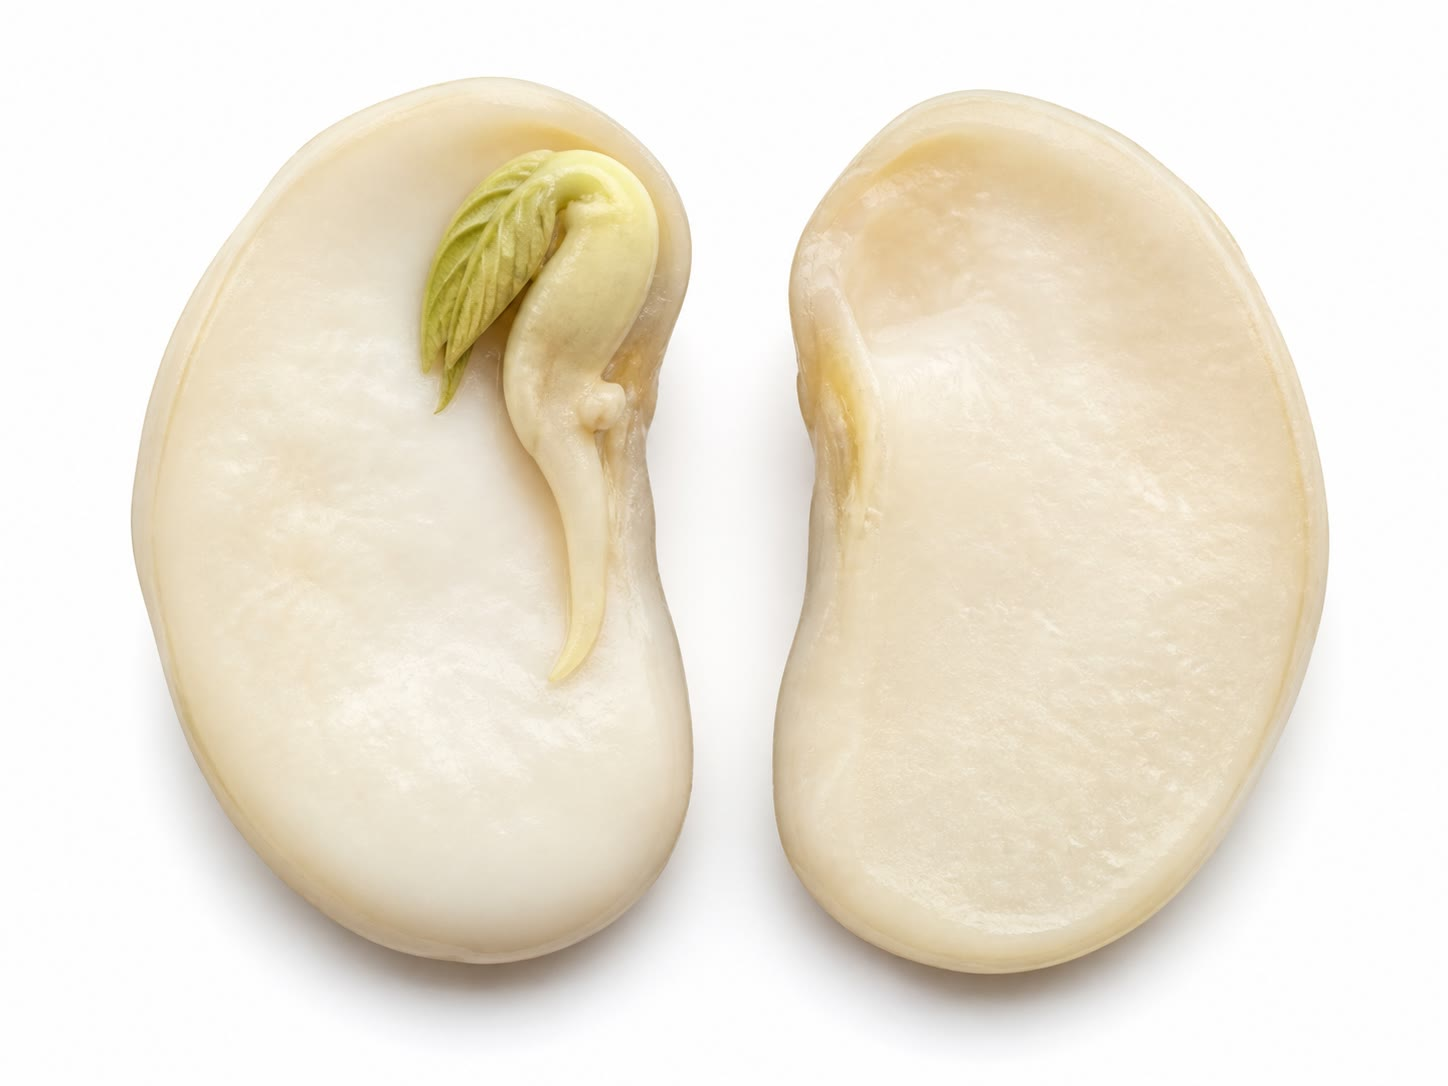
\includegraphics[width=0.62\linewidth]{images/book1/ai/fig-bean-open.jpg}};
  \begin{scope}[x={(img.south east)}, y={(img.north west)},
      every node/.style={font=\small}]
    \draw[omDef, thick] (0.35,0.79) -- (0.26,0.94)
      node[above] {折叠的初生叶};
    \draw[omDef, thick] (0.40,0.38) -- (0.28,-0.04)
      node[below] {根尖};
    \draw[omDef, thick] (0.78,0.35) -- (0.80,-0.04)
      node[below, align=center] {两片厚子叶：\\ 食物储存};
  \end{scope}
\end{tikzpicture}

{\small 泡软、打开后的豆子内部：一株小\omterm{def:g1:plants-around-us:plant}{植物}——根尖
和折叠的初生叶——紧贴着它的食物储存。}
\end{omfigure}

\begin{remark}[种子也在我们的厨房里]\label{rem:g2:from-seed-to-plant:kitchen}
豆子、豌豆、扁豆、大米、葵花籽，还有苹果里的籽
和桃子里的核：厨房里到处都是\omterm{def:g2:from-seed-to-plant:seed}{种子}。有的很小，
像罂粟籽；椰子则是一个大个子。它们每一个，
只要有机会，都会努力长成一株\omterm{def:g1:plants-around-us:plant}{植物}。
\end{remark}

\section{萌发}

\begin{definition}[萌发]\label{def:g2:from-seed-to-plant:germination}
\emph{萌发}\index{萌发}是\omterm{def:g2:from-seed-to-plant:seed}{种子}苏醒并开始生长的时刻：
\omterm{def:g2:from-seed-to-plant:seed}{种子}吸水膨胀，种皮裂开，小根
先长出来并向下扎去，然后芽向上伸展，
带着最初的绿叶朝向光。我们说
\omterm{def:g2:from-seed-to-plant:seed}{种子}\emph{萌发}\index{萌发}了。
\end{definition}

\begin{proposition}[种子萌发需要什么]\label{prop:g2:from-seed-to-plant:needs}
\omterm{def:g2:from-seed-to-plant:seed}{种子}\omterm{def:g2:from-seed-to-plant:germination}{萌发}需要\emph{水}和\emph{温暖}。它暂时
还不需要光：起初，食物储存便养育着\omterm{prop:g2:from-seed-to-plant:cycle}{幼苗}，
即使在土壤之下、黑暗之中。缺水，或处于寒冷之中，
一颗好\omterm{def:g2:from-seed-to-plant:seed}{种子}就只能静静等待。
\end{proposition}
\admitted

\begin{example}[为什么要等到春天才播种]\label{ex:g2:from-seed-to-plant:spring}
园丁在春天而不是冬天播豆种：寒冷的土里，\omterm{def:g2:from-seed-to-plant:seed}{种子}
只会等待——甚至腐烂——而无法\omterm{def:g2:from-seed-to-plant:germination}{萌发}。温暖的日子
与湿润的土壤，正是
\cref{prop:g2:from-seed-to-plant:needs}中的两个信号。
\end{example}

\begin{method}[播种并观察种子萌发]\label{met:g2:from-seed-to-plant:sow}
\begin{enumerate}
  \item 在玻璃罐内壁铺上湿棉花或湿纸；
  \item 把一颗豆子塞进玻璃与棉花之间，好让你看到它；
  \item 把罐子放在温暖的房间里，并保持棉花湿润；
  \item 每天观察并记录所见：豆子膨胀、种皮
        裂开、根向下长、芽向上长。
\end{enumerate}
玻璃让平时在土壤之下发生的事情变得可见。
\end{method}

\begin{omfigure}
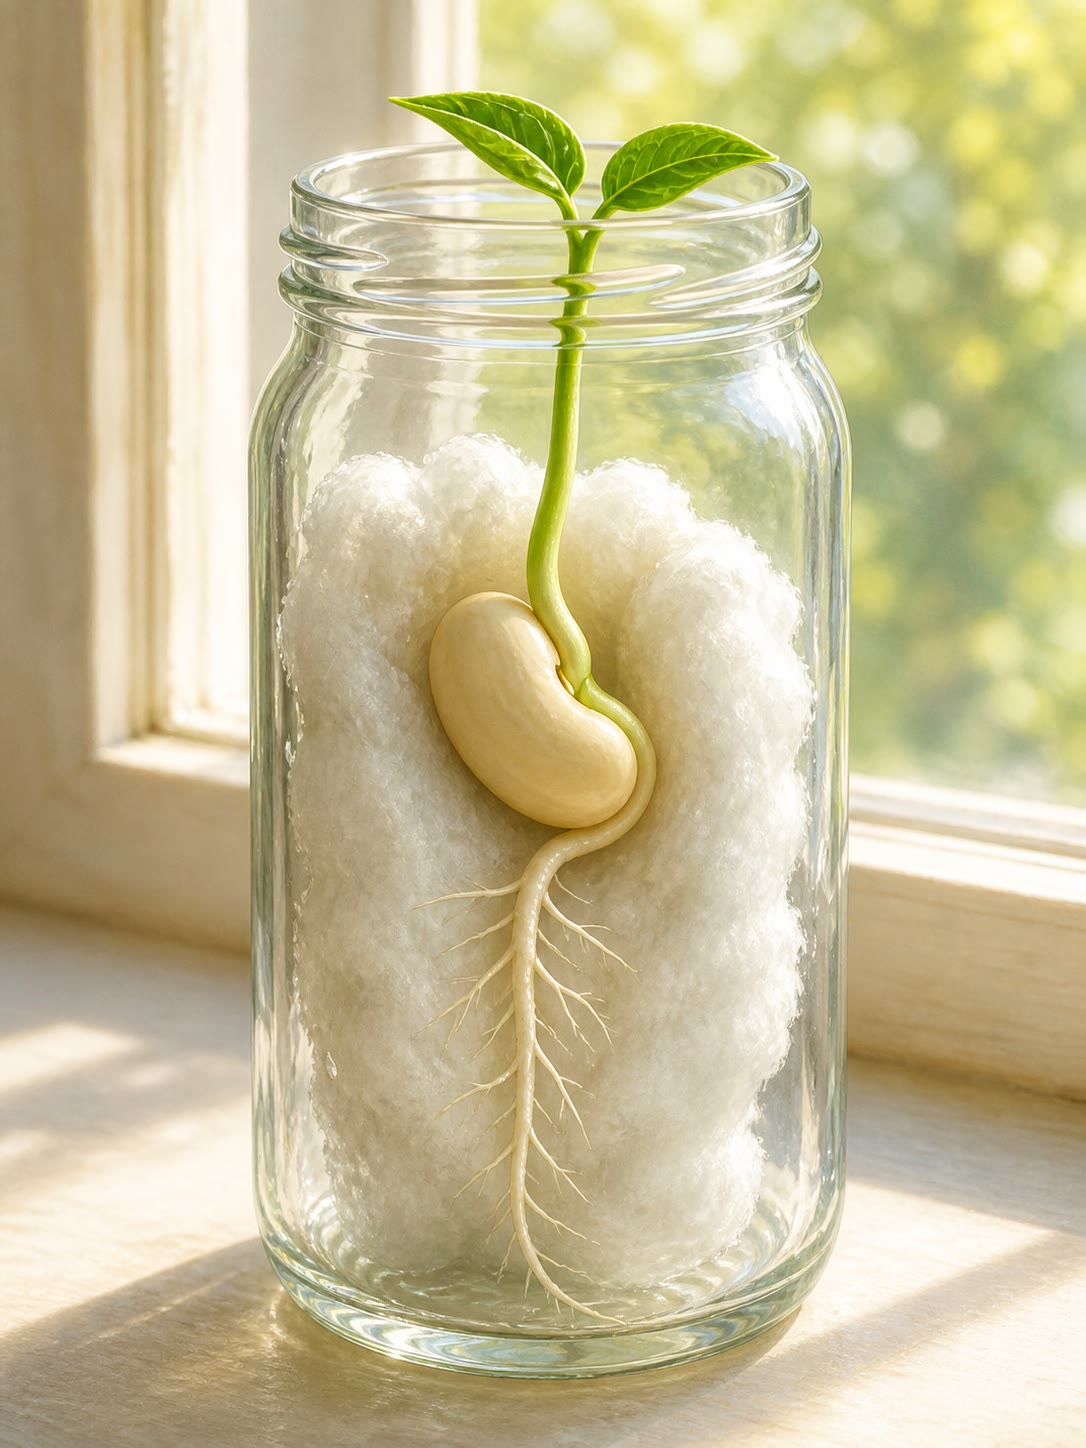
\includegraphics[width=0.44\linewidth]{images/book1/ai/g2-seed-bean-jar.jpg}

{\small 罐中豆子\omterm{def:g2:from-seed-to-plant:germination}{萌发}过程的情形：根向下，芽向上，
两者之间是正在变空的\omterm{def:g2:from-seed-to-plant:seed}{种子}。}
\end{omfigure}

\begin{remark}[根向下，芽向上——始终如此]\label{rem:g2:from-seed-to-plant:updown}
无论豆子在罐中怎样放置——侧躺，或是倒着——
根总是向下转，芽总是向上转。
\omterm{prop:g2:from-seed-to-plant:cycle}{幼苗}看不见，却知道哪边是上。\omterm{def:g1:plants-around-us:plant}{植物}
所感知的，比它们表现出来的要多。
\end{remark}

\section{从幼苗到结出种子的植物}

\begin{proposition}[植物的生命周期]\label{prop:g2:from-seed-to-plant:cycle}
\emph{幼苗}\index{幼苗}长成有根、茎和叶的\omterm{def:g1:plants-around-us:plant}{植物}，
\omterm{def:g1:plants-around-us:plant}{植物}开花；花结出新的
\emph{\omterm{def:g2:from-seed-to-plant:seed}{种子}}，循环便可以重新开始。一株豆子\omterm{def:g1:plants-around-us:plant}{植物}
在一个夏天里就能结出几十颗新豆子。
\end{proposition}
\admitted

\begin{example}[一颗豆子，一个夏天]\label{ex:g2:from-seed-to-plant:summer}
五月播种，一颗豆子一周内就\omterm{def:g2:from-seed-to-plant:germination}{萌发}；到了六月，它已是一株满是\omterm{def:g1:plants-around-us:parts}{叶子}的
\omterm{def:g1:plants-around-us:plant}{植物}，正沿着支架向上攀爬；七月开出白花，随后结出绿色的豆荚；
八月，豆荚沉甸甸地垂挂着，每个豆荚里都藏着一排新豆子
——它们是明年的\omterm{def:g2:from-seed-to-plant:seed}{种子}，由今年这株\omterm{def:g1:plants-around-us:plant}{植物}结出。
\end{example}

\section{练习}

\begin{exercise}[$\star$]\label{exo:g2:from-seed-to-plant:1}
\omterm{def:g2:from-seed-to-plant:seed}{种子}的种皮里面有哪两样东西？
\end{exercise}

\begin{exercise}[$\star$]\label{exo:g2:from-seed-to-plant:2}
\emph{\omterm{def:g2:from-seed-to-plant:germination}{萌发}}是什么意思？\omterm{def:g2:from-seed-to-plant:seed}{种子}里最先长出的
是根，还是幼芽？
\end{exercise}

\begin{exercise}[$\star$]\label{exo:g2:from-seed-to-plant:3}
说出\omterm{def:g2:from-seed-to-plant:seed}{种子}\omterm{def:g2:from-seed-to-plant:germination}{萌发}需要的两个条件。在成年\omterm{def:g1:plants-around-us:plant}{植物}
的常见需要中，哪一项\emph{不}在这张清单上？
\end{exercise}

\begin{exercise}[$\star$]\label{exo:g2:from-seed-to-plant:4}
埋在土中的\omterm{prop:g2:from-seed-to-plant:cycle}{幼苗}，还没见到
光，如何能在黑暗中生长？它最开始的食物从哪里来？
\end{exercise}

\begin{exercise}[$\star$]\label{exo:g2:from-seed-to-plant:5}
说出你能在厨房里找到的四种\omterm{def:g2:from-seed-to-plant:seed}{种子}。
\end{exercise}

\begin{exercise}[$\star$]\label{exo:g2:from-seed-to-plant:6}
园丁为什么要在春季播种，而不在冬季播种？
\end{exercise}

\begin{exercise}[$\star$]\label{exo:g2:from-seed-to-plant:7}
请排序：结有新豆子的豆荚——\omterm{def:g2:from-seed-to-plant:seed}{种子}——开花的\omterm{def:g1:plants-around-us:plant}{植物}——
\omterm{prop:g2:from-seed-to-plant:cycle}{幼苗}——长满\omterm{def:g1:plants-around-us:parts}{叶子}的\omterm{def:g1:plants-around-us:plant}{植物}。
\end{exercise}

\begin{exercise}[$\star$]\label{exo:g2:from-seed-to-plant:8}
动手试一试：用\cref{met:g2:from-seed-to-plant:sow}所用的玻璃罐，
放入两颗豆子：一颗侧放，一颗倒放。\omterm{def:g2:from-seed-to-plant:germination}{萌发}后，
比较它们的根和幼芽。
\cref{rem:g2:from-seed-to-plant:updown}预测了什么结果？
\end{exercise}

\begin{exercise}[$\star\star$]\label{exo:g2:from-seed-to-plant:9}
尼娜把一包豆种放在干燥的抽屉里，整整放了一年，
到她终于播种时，这些\omterm{def:g2:from-seed-to-plant:seed}{种子}仍能\omterm{def:g2:from-seed-to-plant:germination}{萌发}。为什么它们
在抽屉里既没有生长，也没有死去？请利用
\cref{prop:g2:from-seed-to-plant:needs}。
\end{exercise}

\begin{exercise}[$\star\star$]\label{exo:g2:from-seed-to-plant:10}
\cref{ch:g2:animals-grow-up}中的小鸡在卵中长大，
靠卵黄供养。豆子里哪一部分起着卵黄的作用？
卵和\omterm{def:g2:from-seed-to-plant:seed}{种子}有什么共同之处？
\end{exercise}
